%%This is a very basic article template.

\documentclass[a4paper,10pt]{article}
\usepackage{latexsym}
\usepackage{amssymb}
\usepackage{bm}
\usepackage{graphicx}
\usepackage{natbib}
\usepackage{geometry}
\usepackage{pdflscape}
\usepackage{hyperref}


\newgeometry{margin=2cm}
\begin{document}

\title{\flushleft\small{Department Software and Computer Technology\\ 
Faculty EEMCS\\
DELFT UNIVERSITY OF TECHNOLOGY\\}
\center {\Large{Assignment-1 \\
(Tree Pattern Evaluation using SAX)\\
Web Data Management (IN4331)\\
2012-2013}}}
\author{Ioanna Jivet(4259610) \\
Nidhi Singh(4242246) }
        
\date{June 2, 2013}
    
\maketitle

\section{Basic Setup}

For this exercise, we have used two SAX parsers, one which parses the input tree pattern and the other which parses the main XML document
to look for the input tree pattern and find matches. We chose to model the tree-pattern query as an XML and not give it as a string for two main reasons. 
Firstly, we avoided parsing the string and extracting the pattern-tree from it. The parsing of the pattern-tree can be done using a SAX parser.
 And second, the way the input is processed does not influence the execution of the algorithm, so we preferred to focus on the algorithm rather than the input format.

\begin{figure}[h!]
  \centering
    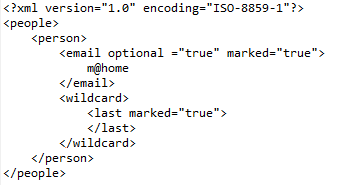
\includegraphics[width=0.5\textwidth]{C:/Users/Nidhi_Chunnu/Documents/GitHub/wdm/Report/pics/pattern_treeXML.png}
    \caption{Pattern-tree XML file}
    \label{fig:pattern}
\end{figure}

As shown in \ref{fig:pattern} the input tree pattern should contain the tree pattern nodes as tags, attributes should be assigned to show if a node is \emph{marked}, or has an 
\emph{optional} edge between its parent. 

\begin{itemize}
  \item \textbf{marked}: takes boolean value \emph{true/false}, default: false
  \item \textbf{optional}: takes boolean value \emph{true/false}, default: false
\end{itemize}

As the XML tag names can�t contain the �*� character to mark a wildcard node, we opted for a keyword �wildcard� to mark such nodes. 
The text within each tag is treated similar to the predicate values in \emph{where} clause of a query. Matched objects are created based on this condition.

\begin{figure}[h!]
  \centering
    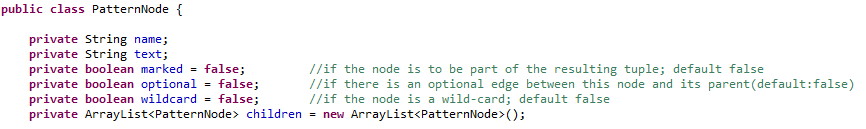
\includegraphics[width=0.95\textwidth]{C:/Users/Nidhi_Chunnu/Documents/GitHub/wdm/Report/pics/patternNode.png}
    \caption{Attributes of PatternNode objects}
    \label{fig:patterncode}
\end{figure}

The pattern-tree is stored in a tree-like structure, where each node is a PatternNode object. \ref{fig:patterncode} shows the attributes of this class. The names of the attributes are self-explanatory. 
The parsing of this XML file into the tree structure is implemented in InputParser.java.

\section{Exercises}
\subsection{Implementation of an evaluation algorithm for C-TP tree-patterns}
\subsubsection{Entities}
The entities of the basic algorithm are abstracted by TPEStack.java, PatterNode.java and Match.java. 
The nodes in the tree-pattern are represented by a PatternNode object. For each node, a TPEStack is created. The stack 
contains all the matches found for the corresponding node. There is a one-to-many relation between the TPEStack and the Match objects. 
Each Match objects contains a reference to its parent Match, the one is linked to, and its child Matches. These references translate 
into the relation between the nested XML nodes in the analyzed XML file. 
\subsubsection{\textbf{TP algorithm}}
 The algorithm is implemented in the StackEval class. By using the SAX parser, the class implements the ContentHandler interface. 
 The parsing of the XML file is done by implementing the startElement(\ldots) and endElement(\ldots) methods. The nodes in the XML file are 
 numbered. The opened tags are monitored through a stack which contains the number of the opened XML element. All the TPEStack are held 
 in a list. They will be used during the execution.
 \begin{itemize}
   \item \textbf{startElement(String uri, String localName, String qName, Attributes attributes)} � when encountering a new tag, the TPEStack list 
   is searched for a TPEStack that corresponds to the node that matches the name of the current opening tag. Additionally, if there exists
an open tag for the parent of this node in the tree-pattern, then the match is valid and added in TPEStack corresponding to the current
 PatternNode. This Match is also linked to parent Matches, to keep the tree structure inside the matches. Next, the attributes of the opened
  tag are checked, in the same manner. Finally, the numbering of the open tags is incremented and the current value is pushed in the open 
  tags stack.
  \item \textbf{endElement(String uri, String localName, String qName)} � when encountering an end tag, the algorithm searches in the list for a TPEStack that corresponds to the node that equals the name of the tag. Again, if there exists an open parent tag and there is a recorded match for this tag, the tag is closed, to keep it in the Match stack inside the TPEStack, but to skip it in following steps. Further pruning is done by checking if the closed Match has all the child Matches, by inspecting the list of children. If at least one child match is missing, the entire match is removed and detached from its parent match.
 \end{itemize}
At the end of the execution, the matches are found in the TPEStack object corresponding to the root PatternNode of the tree-pattern.

\subsection{Implementation of an algorithm that computes the result tuples of C-TP tree patterns}
\subsubsection{\textbf{Tuples extraction algorithm}}
To compute the resulting tuples, the TPEStack associated with the root node of the tree-pattern is traversed. 
For each match in the stack, the tree that results when adding the children matches and their descendants are traversed depth-first 
recursively to obtain the numbers assigned to the matching nodes. In Printer.java, two collection methods are implemented: one for all 
the matching nodes in the tree-pattern, and one only for the marked nodes.
\subsection{Extension to include wildcard ``*'' node}
The wildcard node in the tree-pattern can be substituted for any node in the XML file. Both startElement(\ldots) and endElement(\ldots) methods 
are modified. When opening/closing an XML tag, the list of TPEStacks is searched not only for TPEStacks of the nodes whose name equals 
the name of the tag, but also for a TPEStack that is linked to a node named �wildcard�. This reasoning was explained in the \emph{Basic Setup} section.
\subsection{Extension to include optional nodes}
The optional nodes are denoted by an attribute �optional� in the XML file of the tree-pattern and a field in the PatternNode object. 
The feature is dealt with in the endElement(\ldots) method of the evaluation algorithm. Only the non-optional children of the match 
are checked. The optional child matches are ignored, since it doesn�t matter  if they exist or not.
\subsection{support for predicate values}
To implement this extension, during the SAX parsing of the document, the text between element tags is stored in a HashMap.
 The keys of the map are the numbers associated with each tag. Storing and retrieving the text is easy. The text is collected by 
 implementing the characters(char[] ch, int start, int length) method and adding the found text in the HashMap, using as key the 
 preorder number of the last open tag.
Since the PatternNodes have a field ``text'' that store the value predicate, the only alteration to the algorithm that needs to be 
done is in the endElement(�). Before checking for child matches, the algorithm checks if there exists a value predicate that needs to 
be matched and compares it to the text stored in the Map, at the entry set by the number of the tag.

\subsection{Eextension to return subtrees and not only preorder numbers}
The final extension refers to the formatting of the output: returning subtrees and not only preorder numbers of the tags. 
The algorithm follows the same implementation as the one for extracting the tuples. Instead of adding the preorder numbers, 
they are used to retrieve data from the HashMap that contains the collected text elements. This text is wrapped in the name of 
PatternNode, surrounded by angle brackets.

\subsection{Sample Run}

\subsubsection{Input}
\begin{itemize}
\item tree-pattern  
\begin{figure}[h!]
  \centering
    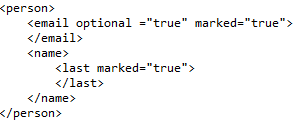
\includegraphics[width=0.5\textwidth]{C:/Users/Nidhi_Chunnu/Documents/GitHub/wdm/Report/pics/tree_pattern.png}
    \caption{Tree-Pattern XML}
    \label{fig:tpattern}
\end{figure}

\item the example from book. 
	\begin{figure}[h!]
  \centering
    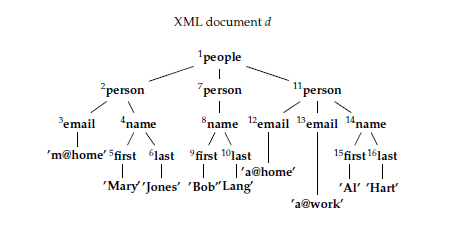
\includegraphics[width=0.5\textwidth]{C:/Users/Nidhi_Chunnu/Documents/GitHub/wdm/Report/pics/XMLexample.png}
    \caption{Book Example}
    \label{fig:example}
\end{figure}

\end{itemize}

\subsubsection{Output}
Figure \ref{fig:result} shows the obtained results
	\begin{figure}[h!]
  \centering
    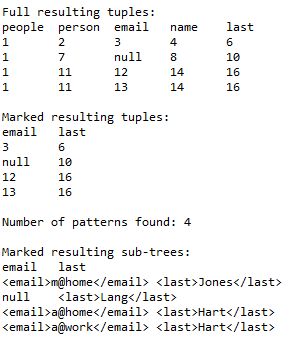
\includegraphics[width=0.5\textwidth]{C:/Users/Nidhi_Chunnu/Documents/GitHub/wdm/Report/pics/results.png}
    \caption{Result snippet}
    \label{fig:result}
\end{figure}
\end{document}